% !TEX encoding = UTF-8 Unicode
\documentclass[a4paper]{article}

\usepackage{color}
\usepackage{url}
\usepackage[T2A]{fontenc} % enable Cyrillic fonts
\usepackage[utf8]{inputenc} % make weird characters work
\usepackage{graphicx}
\usepackage{mathtools}
\usepackage{amsmath}
\usepackage[english,serbian]{babel}
\usepackage{comment}
\usepackage{multirow}
\usepackage[svgnames,table,xcdraw]{xcolor}
\usepackage{tikz}
\usepackage{longtable}
\usepackage{changepage}
\usepackage{setspace}
\usepackage{hhline}
\usepackage{multicol}
\usepackage{tabto}

\usepackage{geometry}
\usepackage{minted}
\usemintedstyle{borland}

%\usepackage[english,serbianc]{babel} %ukljuciti babel sa ovim opcijama, umesto gornjim, ukoliko se koristi cirilica

\usepackage[unicode]{hyperref}
\hypersetup{colorlinks,citecolor=green,filecolor=green,linkcolor=blue,urlcolor=blue}

\usepackage{listings}

%\newtheorem{primer}{Пример}[section] %ćirilični primer
\newtheorem{primer}{Primer}[section]

\definecolor{mygreen}{rgb}{0,0.6,0}
\definecolor{mygray}{rgb}{0.5,0.5,0.5}
\definecolor{mymauve}{rgb}{0.58,0,0.82}

\lstset{ 
  backgroundcolor=\color{white},   % choose the background color; you must add \usepackage{color} or \usepackage{xcolor}; should come as last argument
  basicstyle=\scriptsize\ttfamily,        % the size of the fonts that are used for the code
  breakatwhitespace=false,         % sets if automatic breaks should only happen at whitespace
  breaklines=true,                 % sets automatic line breaking
  captionpos=b,                    % sets the caption-position to bottom
  commentstyle=\color{mygreen},    % comment style
  deletekeywords={...},            % if you want to delete keywords from the given language
  escapeinside={\%*}{*)},          % if you want to add LaTeX within your code
  extendedchars=true,              % lets you use non-ASCII characters; for 8-bits encodings only, does not work with UTF-8
  firstnumber=1000,                % start line enumeration with line 1000
  frame=single,	                   % adds a frame around the code
  keepspaces=true,                 % keeps spaces in text, useful for keeping indentation of code (possibly needs columns=flexible)
  keywordstyle=\color{blue},       % keyword style
  language=Python,                 % the language of the code
  morekeywords={*,...},            % if you want to add more keywords to the set
  numbers=left,                    % where to put the line-numbers; possible values are (none, left, right)
  numbersep=5pt,                   % how far the line-numbers are from the code
  numberstyle=\tiny\color{mygray}, % the style that is used for the line-numbers
  rulecolor=\color{black},         % if not set, the frame-color may be changed on line-breaks within not-black text (e.g. comments (green here))
  showspaces=false,                % show spaces everywhere adding particular underscores; it overrides 'showstringspaces'
  showstringspaces=false,          % underline spaces within strings only
  showtabs=false,                  % show tabs within strings adding particular underscores
  stepnumber=2,                    % the step between two line-numbers. If it's 1, each line will be numbered
  stringstyle=\color{mymauve},     % string literal style
  tabsize=2,	                   % sets default tabsize to 2 spaces
  title=\lstname                   % show the filename of files included with \lstinputlisting; also try caption instead of title
}

\begin{document}

\title{Razvoj rekurentne neuronske mreže i primena na analizi vremenskih serija\\  \small{Seminarski rad u okviru kursa\\Računarska inteligencija\\ Matematički fakultet}}

\author{Kristina Pantelić, 91/2016, kristinapantelic@gmail.com \\Nevena Mesar, 107/2015, mi15107@alas.matf.bg.ac.rs }

%\date{.}

\maketitle

\abstract{
Danas je upotreba neuronskih mreža za rešavanje diverziteta računarskih problema u širokoj upotrebi. Za različite probleme koriste se različite vrste neuronskih mreža. U ovom radu čitalac će se upoznati sa terminom neurona, neuronske mreže, rekurentne neuronske mreže i primenom rekurentne neuronske mreže na analizi vremenskih serija.
}

\tableofcontents

\newpage

\section{Uvod}
\label{sec:uvod}

Algoritmi neuronskih mreža su nastali kao pokušaj da se oponaša način na koji ljudski
mozak uči tj. način na koji ljudski mozak klasifikuje i spoznaje stvari. Neuronske mreže su razvijene tako da simuliraju neurone tj. mreže neurona mozga\cite{master_rad}. U tradicionalnoj neuronskoj mreži svi ulazi i izlazi su nezavisni jedni od drugih, ali u slučajevima kada se, na primer, zahteva predviđanje sledeće reči u rečenici, zahteva se da imamo informaciju o prethodnoj reči i da je na neki način zapamtimo\cite{introRNN}. Ovaj problem je bio motivacija za pojavljivanje i razvijanje rekurentne neuronske mreže. Rekurentna neuronska mreža (RNN) ima "memoriju"{} koja pamti sve informacije koje je prethodno izračunala tj. naučila. Treba imati na umu da tradicionalna neuronska mreža takođe pamti informacije, ali samo one koje je naučila tokom treninga. Na primer, ako klasifikator nauči zavisnosti ulaznih od izlaznih podataka tokom treninga, koristiće to znanje da klasifikuje test instance. Dok RNN takođe uči prilikom treninga, dodatno, ona pamti informacije naučene iz prethodnih trening instanci da bi generisala izlazne podatke\cite{introRNN2}. Ovo svojstvo pamćenja informacija kroz vreme omogućava RNN mreži predikciju u oblasti vremenskih serija\cite{introRNN}, kojima u ovom radu posvećujemo pažnju u kontekstu primene RNN. \\
\indent Na samom početku ovog rada upoznaćemo se sa modelom naše rekurentne neuronske mreže, a u daljem tekstu ćemo se upoznati sa korišćenim skupom podataka vremenskih serija i primenom RNN na skup.  


\section{Rekurenta neuronska mreža}
\label{sec:model}

Postoji više vrsta neuronskih mreža koja, svaka zbog svojih specifičnih karakteristika, daju dobre rezultate na specifičnim poljima istraživanja podataka. Vrsta mreže koja je tema našeg rada je rekurentna neuronska mreža, a naša koncentracija je na razvijanju Jordanove strukturne rekurentne neuronske mreže (eng. \textit{Jordan SRNN}).\\
\indent Jordanova rekurentna neuronska mreža je zasnovana na konceptu koji podrazumeva ponovno korišćenje dobijenih izlaznih vrednosti mreže kao dodatnih informacija za usmeravanje pretrage i izračunavanje novih vrednosti rezultata. Pored ulaznih instanci, dodaju se novih $k$ vrednosti koje predstavljaju vrednosti $k$ rezultata. Dakle, kopija izlaznog sloja se sprovodi na ulaz.\\
%Rekurentna neuronska mreža kojoj posvećujemo pažnju je Jordanova rekurentna neuronska mreža. 
\indent Naš cilj je konstruisati rekurentu neuronsku mrežu sa jednim skrivenim slojem koja će za 6 unetih uzastopnih dana prognozirati količinu padavina za 7. dan. U nastavu ćemo predstaviti model ove mreže u skladu sa brojem naših izlaznih vrednosti (jedan izlazni podatak) i odgovarajuće oznake korišćene u k\^{o}du za implementaciju mreže.

\subsection{Model rekurentne neuronske mreže}
\label{sec:model}

Neuronska mreža se sastoji od 3 sloja koju čine ulazni, skriveni i izlazni sloj. Svaki od slojeva ima odgovarajući broj neurona tj. promenljivih.
Ulazni sloj se sastoji od $n+p$ ulaznih promenljivih $x^{(l)}_1$, $x^{(l)}_2$, ..., $x^{(l)}_n$,$o^{(l-1)}_1$, $o^{(l-1)}_2$, …, $o^{(l-1)}_p$,  uz dodatnu promeljivu $x^{(l)}_0$, koja se naziva bajes i čija je vrednost uvek jednaka 1, za svako $l$. Promenljiva $l$ u superskriptu promenljive $x_i$ predstavlja redni broj instance u skupu odabranih instanci za treniranje mreže. Radi jednostavnosti sve ulazne promenljive označavamo sa $x_i {}\in{}[ \,0,n+p ] \,$. Skriveni sloj čine $m$ neurona $h^{(l)}_1$, $h^{(l)}_2$, …, $h^{(l)}_m$ uz dodatnu promenljivu $h^{(l)}_0=1$, za svako $l$, koja predstavlja bajes za skriveni sloj mreže. Izlazni sloj čine $p$ neurona, čiji su izlazi $o^{(l)}_1$, $o^{(l)}_2$, …, $o^{(l)}_p$. Svi neuroni ulaznog sloja su spojeni sa svim neuronima skrivenog sloja, osim bajesa, vezama čije su težine $w’_{ij}$, $0\leq{}i\leq{}n+p$, $0\leq{}j\leq{}m$. Svi neuroni skrivenog sloja su povezani sa svim neuronima izlaznog sloja vezama sa težinama $w{''}_{jk}$, $0\leq{}j\leq{}m$, $1\leq{}k\leq{}p$. 

Nakon završavanja algoritma, cilj je da izlazne vrednosti budu što bliže izlaznim vrednostima $y_1$, $y_2$,...,$y_p$.

\begin{figure}[h!]
\begin{center}
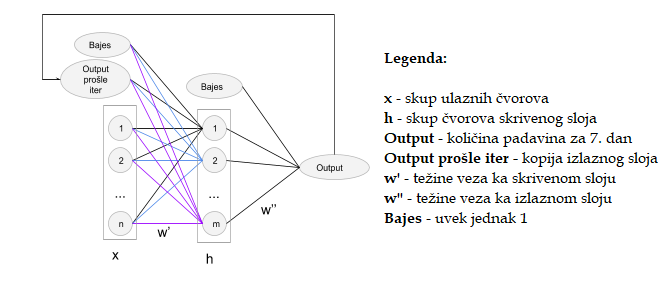
\includegraphics[scale=0.7]{net.png}
\end{center}
\caption{Jordanova RNN sa jednim skrivenim slojem}
\end{figure}

Proces učenja se sastoji od više iteracija, gde se svaka iteracija izvršava u nekoliko koraka. Najpre se, za sve $j$, $1\leq{}j\leq{}m$, izračunava vrednost:

\begin{equation}
u'_j = \sum_{i=0}^{n+p}x_iw'_{ij}
\end{equation}
 
i $h_j= f(u'_j)$, gde je $f(x)=(1+e^{-x})^{-1}$ sigmoidna funkcija. Sigmoidna funkcija predstavlja aktivacionu funkciju neurona skrivenog i izlaznog sloja. Analogno kao kod skrivenog sloja, određuju se vrednosti izlaza iz neurona izlaznog sloja. Tako se dobija 

\begin{equation}
u{''}_k = \sum_{ij=0}^{m}h_jw{''}_{jk}
\end{equation}
 
i $o_k= f(u{''}_k)$. Nakon odgovarajućeg broja iteracija, očekujemo da će vrednosti $o_k$ biti približno jednake željenim izlaznim vrednostima $y_k$.
Greška izlaznog sloja neurona k je definisana:

\begin{equation}
E_k = \frac{1}{2}(y_k - o_k)^2.
\end{equation}

Pri ažuriranju vrednosti $w{''}_{jk}$, važi $w{''}_{jk}=w{''}_{jk}+w{''}_jk$, gde je
$$\Delta{} w{''}_{jk}=- \eta{}\frac{\partial{}E_k}{\partial{}w{''}_{jk}}+\alpha{}w{''}_{jk}.$$

Parametri $\eta{}$ i $\alpha{}$, respektivno, mere uticaj parcijalnog izvoda greške $E_k$ po $w{''}_{jk}$ i prethodne vrednosti $w{''}_{jk}$. Kako je $E_k$ funkcija od $o_k$, $o_k$ funkcija od $u{''}_k$, a $u{''}_k$ funckija čiji je jedan od argumenata $w{''}_{jk}$, prema pravilu o izvodu složene funkcije važi 

$$\frac{\partial{}E_k}{\partial{}w{''}_{jk}} = \frac{\partial{}E_k}{\partial{}o_{k}}\frac{\partial{}o_k}{\partial{}u{''}_{k}}\frac{\partial{}u{''}_k}{\partial{}w{''}_{jk}} = -(y_k-o_k)f'(u{''}_k)h_j = -(y_k-o_k)o_k(1-o_k)h_j$$

Iz poslednjeg reda sledi da je 

$$\Delta{}w{''}_{jk}=\eta{}(y_k-o_k)o_k(1-o_k)h_j+\alpha{}w{''}_{jk}$$

Greška neurona skrivenog sloja predstavlja sumu svih odgovarajućih grešaka neurona izlaznog sloja i određena je sa

$$E_j = \frac{1}{2}\sum_{k=1}^p(y_k - o_k)^2$$.

Pri ažuriranju vrednosti $w'_{ij}$, važi $w'_{ij}=w'_{ij} + \Delta{}w'_{ij}$, gde je

$$\Delta{}{}w'_{ij} = - \eta{}\frac{\partial{}E_j}{\partial{}w{'}_{ij}}+\alpha{}w'_{ij}$$.

Vrednost $\frac{\partial{}E_j}{\partial{}w'_{ij}}$ se može izračunati prema pravilu o izvodu složene funkcije na sledeći način:

$$\frac{\partial{}E_j}{\partial{}w'_{ij}}=\frac{\partial{}E_j}{\partial{}o_{k}}\frac{\partial{}o_k}{\partial{}u{''}_{k}}\frac{\partial{}u{''}_k}{\partial{}h_{j}}\frac{\partial{}h_j}{\partial{}u'_{j}}\frac{\partial{}u'_j}{\partial{}w'_{ij}}$$
$$ = -\sum_{k=1}^p(y_k-o_k)f'(u{''}_k)w{''}_{jk}f'(u'_j)x_i$$
$$ = -\sum_{k=1}^p(y_k-o_k)o_k(1-o_k)w{''}_{jk}h_j(1-h_j)x_i$$

Sledi da je 
$$\Delta{}w'_{ij}=\eta{}x_ih_j(1-h_j)\sum_{k=1}^p(y_k-o_k)o_k(1-o_k)w{''}_{jk} + \alpha{}\Delta{}w'_{ij}\cite{model}$$

\subsection{Algoritam rekurentne neuronske mreže}
\label{sec:model}

Na osnovu prethodnog opisa, algoritam učenja se izvršava u sledećih osam koraka\cite{model}:

\begin{enumerate}
  \item Ulazni podaci se sastoje od parova vektora ($x^{(l)}_1$, $x^{(l)}_2$,..., $x^{(l)}_{n+p}$) i ($y_1$, $y_2$,..., $y_p$), gde $x_i$ predstavljaju ulaze uključujući kopiju rezultata iz prethodne iteracije algoritma, a $y_k$ željene izlaze za svaku ulaznu instancu. Skup ulaznih podataka se proširuje bajesom $x^{(l)}_0=1, {}\forall{l}$ iz skupa podataka.
  \item Inicijalizovati parametre $\eta{}$, $\alpha{}$ i odrediti kriterijum zaustavljanja. Inicijalizovati početne vrednosti za $w'_{ij}$ i $w{''}_{jk}$ i postaviti $\Delta{}w'_{ij}=\Delta{}w{''}_{jk}=0$. Izabrati aktivacionu funkciju f (ovde je korišćena sigmoidna funkcija).
  \item Izabrati novi par ulaznog i izlaznog vektora (novi test primer iz skupa za učenje).
  \item Odrediti vrednosti $u'_j$ i $h_j$. Postaviti $h^{(l)}_0=1, {}\forall{l}$ iz skupa podataka.
  \item Odrediti vrednosti $u{''}_k$ i $o_k$. Ukoliko je ispunjen kriterijum zaustavljanja, prekinuti izvršavanje.
  \item Odrediti $\Delta{}w{''}_{jk}$ i ažurirati vrednosti $w{''}_{jk}$.
  \item Odrediti $\Delta{}w{'}_{ij}$ i ažurirati vrednosti $w{'}_{ij}$.
  \item Preći na korak 3.
\end{enumerate}

% ----------------------------------------------------------------------- IMPLEMENTACIJA

\section{Implementacija algoritma}

U primerima metoda izostavljene su metode korišćenje za logovanje.

\subsection{Potrebne biblioteke}
Za implementaciju algoritma oslonili smo se na neke od funkcionalnosti postojećih biblioteka:
\begin{itemize}
    \item \texttt{numpy} -- kako bismo optimizovali matrične operacije
    \item \texttt{pandas} -- za ucitavanje i manipulisanje skupom podataka
    \item \texttt{sklearn} -- za podelu podataka na test i trening skup, predprocesiranje podataka i ocenu greški
    \item \texttt{matplotlib} -- za iscrtavanje grafika
\end{itemize}

\begin{minted}{python}
from sklearn.metrics import mean_absolute_error, mean_squared_error
from sklearn.model_selection import train_test_split
from sklearn.preprocessing import MinMaxScaler
from pandas import DataFrame, Series, read_csv, errors, concat, Grouper
from numpy import zeros, array, append, concatenate, multiply, vstack, matrix, around
from numpy.random import rand, seed
from matplotlib import pyplot as plt
\end{minted}

\subsection{Podaci i predprocesiranje}
Podaci su preuzeti sa \href{https://www.meteoblue.com/en/weather/archive/export/basel_switzerland_2661604}{Meteo blue}, za Švajcarski grad Basel. Skup podataka je namerno izabran tako da su nema nedostajućih podataka i da su svi dani u kontinuitetu. U realnosti to ne bi bio slučaj. Ovaj rad ne obuhvata obradu takvih slučajeva, ali je jedan od mogućih koraka za unapređenje projekta.
\\
U pitanju je period počev od datuma 31.12.1990. do 31.12.2019, ukupno 11326 uzastopnih dana.
Skup svih atributa koji su dostupni u originalnom skupu podataka se može videti u tabeli \ref{tab:atributi}. Uklonjeni su atributi koji su osenčeni sivom pozadinom. Odlučili smo da ih uklonimo radi brzine izračunavanja, moguće ih je uključivati u cilju eksperimentisanja. \texttt{Timestamp} smo izbacili jer su podaci učitavani hronološki, pa je samim tim indeks u skupu podataka dovoljan.

\begin{table}[h]
\begin{tabular}{|l|l|l|l|l|}
\hline
\rowcolor[HTML]{EFEFEF} 
Timestamp               &          &                         &       &           \\ \hline
Temperature             & \textcelsius       & 2 m elevation corrected & daily & Minimum   \\ \hline
Temperature             & \textcelsius       & 2 m elevation corrected & daily & Maximum   \\ \hline
Temperature             & \textcelsius       & 2 m elevation corrected & daily & Mean      \\ \hline
\rowcolor[HTML]{EFEFEF} 
Relative Humidity       & \%       & 2 m                     & daily & Minimum   \\ \hline
\rowcolor[HTML]{EFEFEF} 
Relative Humidity       & \%       & 2 m                     & daily & Maximum   \\ \hline
Relative Humidity       & \%       & 2 m                     & daily & Mean      \\ \hline
Precipitation Total     & mm       & sfc                     & daily & Summation \\ \hline
Cloud Cover Total       & \%       & sfc                     & daily & Mean      \\ \hline
Evapotranspiration      & mm       & sfc                     & daily & Summation \\ \hline
\rowcolor[HTML]{EFEFEF} 
Wind Speed              & km/h     & 10 m                    & daily & Minimum   \\ \hline
\rowcolor[HTML]{EFEFEF} 
Wind Speed              & km/h     & 10 m                    & daily & Maximum   \\ \hline
Wind Speed              & km/h     & 10 m                    & daily & Mean      \\ \hline
\rowcolor[HTML]{EFEFEF} 
Wind Direction Dominant & \textdegree        & 10 m                    & daily & None      \\ \hline
\rowcolor[HTML]{EFEFEF} 
Temperature             & \textcelsius       & sfc                     & daily & Minimum   \\ \hline
\rowcolor[HTML]{EFEFEF} 
Temperature             & \textcelsius       & sfc                     & daily & Maximum   \\ \hline
\rowcolor[HTML]{EFEFEF} 
Temperature             & \textcelsius       & sfc                     & daily & Mean      \\ \hline
\rowcolor[HTML]{EFEFEF} 
Soil Temperature        & \textcelsius       & 0-10 cm down            & daily & Minimum   \\ \hline
\rowcolor[HTML]{EFEFEF} 
Soil Temperature        & \textcelsius       & 0-10 cm down            & daily & Maximum   \\ \hline
Soil Temperature        & \textcelsius       & 0-10 cm down            & daily & Mean      \\ \hline
\rowcolor[HTML]{EFEFEF} 
Soil Moisture           & fraction & 0-10 cm down            & daily & Minimum   \\ \hline
\rowcolor[HTML]{EFEFEF} 
Soil Moisture           & fraction & 0-10 cm down            & daily & Maximum   \\ \hline
Soil Moisture           & fraction & 0-10 cm down            & daily & Mean      \\ \hline
\rowcolor[HTML]{EFEFEF} 
Vapor Pressure Deficit  & hPa      & 2 m                     & daily & Minimum   \\ \hline
\rowcolor[HTML]{EFEFEF} 
Vapor Pressure Deficit  & hPa      & 2 m                     & daily & Maximum   \\ \hline
\rowcolor[HTML]{EFEFEF} 
Vapor Pressure Deficit  & hPa      & 2 m                     & daily & Mean      \\ \hline
\end{tabular}
\caption{Dostupni atributi, osenčeni se ne koriste}
\label{tab:atributi}
\end{table}
Atributi su preimenovani tako da im je dodeljen kraći naziv. Ciljni atribut je \texttt{precipitation}, dok su ostali korišćeni za predviđanje. 
\begin{minted}{python}
colnames = {
    "Basel Temperature [2 m elevation corrected]": "tempMin",
    "Basel Temperature [2 m elevation corrected].1": "tempMax",
    "Basel Temperature [2 m elevation corrected].2": "tempMean",
    # "Basel Relative Humidity [2 m]": "rHumidMin",
    # "Basel Relative Humidity [2 m].1": "rHumidMax",
    "Basel Relative Humidity [2 m].2": "rHumidMean",
    "Basel Precipitation Total": "precipitation",
    "Basel Cloud Cover Total": "cloudCoverage",
    "Basel Evapotranspiration": "evapor",
    # "Basel Wind Speed [10 m]": "windSpeedMin",
    # "Basel Wind Speed [10 m].1": "windSpeedMax",
    "Basel Wind Speed [10 m].2": "windSpeedMean",
    # "Basel Soil Temperature [0-10 cm down]": "soilTempMin",
    # "Basel Soil Temperature [0-10 cm down].1": "soilTempMax",
    "Basel Soil Temperature [0-10 cm down].2": "soilTempMean",
    # "Basel Soil Moisture [0-10 cm down]": "soilMoistMin",
    # "Basel Soil Moisture [0-10 cm down].1": "soilMoistMax"
    "Basel Soil Moisture [0-10 cm down].2": "soilMoistMean"
}
\end{minted}

 Podaci su podeljeni na test i trening skup u razmeri $3:7$, skup za test ima 3398 redova, dok je za trening korišćeno 7928 redova. Za podelu je korišćena \texttt{test\_train\_split} metoda iz \texttt{sklearn.model\_selection}.


\begin{minted}{python}
def test_train_split_mine():
    global df, x_train, y_train, x_test, y_test, test_size
    global g_y_colname, n_x_test, n_x_train
    Y = df[g_y_colname]
    X = df.drop(columns=[g_y_colname])
    x_train, x_test, y_train, y_test = train_test_split(
        X, Y, shuffle=False, test_size=test_size)
    n_x_train = x_train.shape[0]
    n_x_test = x_test.shape[0]
    x_test.reset_index(inplace=True, drop=True)
    y_test.reset_index(inplace=True, drop=True)
\end{minted}

Izvršeno je skaliranje podataka pomoću \texttt{MinMaxScaler} iz \texttt{sklearn.preprocessing} modula tako da sve vrednosti upadnu u rang $[0.1, 0.9]$. Skaliranje testnog skupa vršilo se na osnovu skupa za trening. Ciljni atribut je takođe skaliran na taj interval sa intervala $[0, 100]$.

\begin{minted}{python}
def scale_attributes():
    global x_train, x_test, y_train, y_test
    scaler = MinMaxScaler(feature_range=(0.1, 0.9))
    scaler.fit(x_train, y_train)
    x_train = scaler.transform(x_train)
    x_test = scaler.transform(x_test)

    y_train = f_scale_y(y_train)
    y_test = f_scale_y(y_test)
\end{minted}

\subsection{Treniranje mreže}

Kao aktivacionu funkciju koristimo sigmoidnu funkciju.
\begin{minted}{python}
def activation_f(u):
    return 1.0 / (1.0 + exp(-u))
\end{minted}

\subsubsection{Inicijalizacija}
Za početak je potrebno inicijalizovati matrice težina i njihove derivate. Težinske matrice su popunjene proizvoljnim vrednostima. Naglasiti da je prva iteracija zbog dodavanja izlaznog čvora, i definisati kroz koliko paterna treba da prođemo. 
\begin{minted}{python}
init_iter = True
n = N * n_attrs + 1     # broj ulaznih cvorova + 1 za bias
n_x = len(x_train)
num_of_patterns = n_x - N
m += 1                  # broj cvorova skrivenog sloja + bias
w_ = rand(n, m) - 0.5
dw_ = zeros((n, m))
w__ = rand(m) - 0.5     # samo jedan output -> obican niz
dw__ = zeros(m)
o = zeros(num_of_patterns)
output_arr = array([])
day = 0
end_of_epoch = n_x - N - 1
\end{minted}
Treniranje je realizovano kroz epohe. Jedna epoha predstavlja jedan prolazak kroz celokupan skup za trening. Na kraju svake epohe računaju se greške pomoću \texttt{mean\_absolute\_error}, \texttt{mean\_squared\_error} iz \texttt{sklearn.metrics}, kao i  \texttt{root squared error} dobijena od \texttt{mse} i prikazuju na izlazu. Trenira se dok se ne dostigne maksimalan broj epoha koji je 20. Takođe, u prvoj epohi, središnjoj i poslednjoj pravi se grafik koji prikazuje prave vrednosti i predviđene za poslednjih 365 dana epohe. Za sve predviđene vrednosti koje su skalirane na pravu vrednost dale negativan broj smatraćemo da su $0$.

Podrazumevane vrednosti parametara su $ \eta{} = 0.3$ i $\alpha{} = 0.2 $. Prilikom pokretanja programa moguće je postaviti ih na druge vrednosti.

Za broj čvorova skrivenog sloja testirano je par varijanti. Ostavljeno je da se računa po formuli:
\begin{minted}{python}
m = (int)((N * n_attrs) * 4)
\end{minted}

\subsubsection{Koraci algoritma}
Cilj je konstruisati neuronsku mrežu sa jednim skrivenim slojem koja će za 6 unetih uzastopnih dana prognozirati količinu padavina za 7. dan. Ideja korišćena kako bi se podaci maksimalno iskoristili je prikazana na slici \ref{fig:dani}.

\begin{figure}[h]
\begin{center}
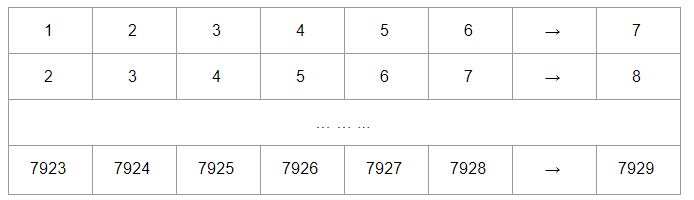
\includegraphics[scale=0.7]{dani.JPG}
\end{center}
\caption{Paterni za treniranje mreže}
\label{fig:dani}
\end{figure}

Ulazni čvorovi su svi atributi 6 uzastopnih dana, tako da su dani jedan za drugim u nizu i poštuje se redosled atributa. Na prvom mestu je uvek bias, dok se na kraj dodavao izlaz prethodne iteracije. U prvoj, inicijalnoj iteraciji, izlazni čvor ne postoji pa se dodavala prazna lista.
\begin{minted}{python}
input_nodes = concatenate((bias, 
                          (x_train[day:(day+N)]).reshape(-1), 
                          output_arr))
\end{minted}

U nastavku biće prikazana naivna implementacija i koraci kojima se došlo do sažimanja operacija i njihovog prevođenja u matrične i vektorske operacije biblioteke \texttt{numpy}. Odlučili smo da iskoristimo \texttt{numpy} biblioteku radi optimizacije vremenske slozenosti osnovnih operacija algoritma.

\paragraph{Izracunavanje h1,..., hm cvorova skrivenog sloja}
\begin{minted}{python}
# Naivna implementacija
h[0] = 1.0
for j in range(1, m+1):
    u = 0
    for i in range(0, n+1):
        u += input_nodes[i] * w_[i][j]
    h[j] = activation_f(u)
\end{minted}

Proces dolaska do poboljšane implementacije se svodi na sledeće interpretiranje naivne: \\
{\it Za svaku kolonu težinske matrice pokoordinatno pomnoži kolonu sa ulaznim čvorovima, dobijene vrednosti sumiraj i provuci kroz aktivacionu funkciju.} Umesto da se fokusiramo na pojedinačne elemente matrice uopštili smo postupak koristeći osobine matrica i vektora. Grafički to možemo predstaviti na primeru manje dimenzije prikazanom na slici \ref{fig:izracunavanjewp}.

\begin{figure}[h!]
    \subfigure{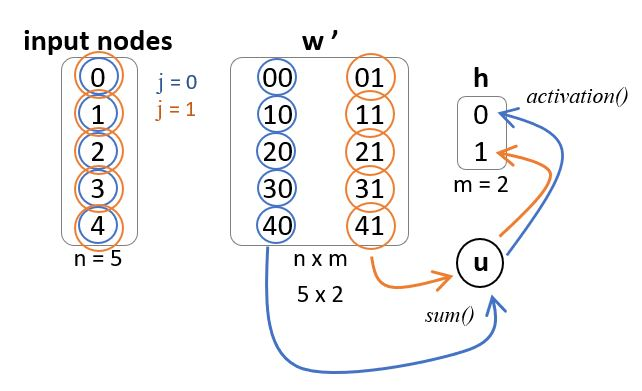
\includegraphics[width=0.48\linewidth]{naivno_izracunavanje_w_.JPG}}
    \subfigure{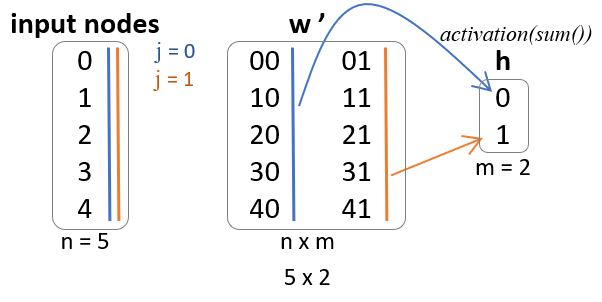
\includegraphics[width=0.48\linewidth]{izracunavanje_w_.JPG}} 
    \caption{Primeri izračunavanja vrednosti čvorova skrivenog sloja. Naivni pristup sa leve i pristup koji koristi vektorske operacije sa desne strane.}
    \label{fig:izracunavanjewp}
\end{figure}

\texttt{numpy} funkcija \texttt{multiply} radi pokoordinatno množenje koje nama u ovom slučaju treba. Takođe, bilo je potrebno transponovati težinsku matricu kako bi se dimenzije poklopile, i atributi množili svojim težinama. Prednost petlje u \texttt{python}-u jeste to što iterira po redovima, pa samim tim možemo automatski proći kroz težinsku matricu.
Konačno dobijamo poboljšanu verziju ovog koraka:
\begin{minted}{python}
# Poboljsana implementacija
u = []
for i in w_.T:
    u += [activation_f(sum(multiply(i, input_nodes)))]
h = array(u)
h[0] = 1  # bias ostaje nepromenjen
\end{minted}

\paragraph{Izracunavanje o1,...,op}
\begin{minted}{python}
# Naivna implementacija
for k in range(1, p+1):
    u = 0
    for j in range(0, m+1):
        u += h[j] * w__[j][k]
    o[day] = activation_f(u)
\end{minted}
U prvobitnoj implementaciji $w''$ težinsku matricu smo posmatrali kao matricu, kasnije smo sveli na niz pošto imamo samo jedan izlazni čvor, pa prema tome nema potrebe praviti matricu. Koristi se isti princip kao u prethodnom koraku, pokoordinatno se pomnože skriveni čvorovi sa težinskim vektorom u ovom slučaju, sumiraju se dobijeni rezultati i provuku kroz aktivacionu funkciju.
\begin{minted}{python}
# Poboljsana implementacija
o[day] = activation_f(sum(multiply(h, w__)))
output_arr = array([o[day]])
\end{minted}

\paragraph{Greška}
Greška je broj koji se pojavljuje u izračunavanju na više mesta: prilikom računanja \texttt{dh} i ažuriranja \texttt{dw\_\_}. Zato je pogodno izdvojiti je u posebnu promenljivu i nadalje je koristiti.
\begin{minted}{python}
error = (y_train[day+N] - o[day]) * o[day] * (1.0 - o[day])
\end{minted}

\paragraph{Izracunavanje deltaH(j)}
\begin{minted}{python}
# Naivna implementacija
for j in range(1, m+1):
    dh[j] = 0.0
    for k in range(1, p+1):
        dh[j] += w__[j][k] * error
\end{minted}
Umesto resetovanja vrednosti i njihovog ponovnog izračunavanja u postojećoj \texttt{dh}, možemo direktno iskoristiti vrednosti $w''$ težinskog vektora u našem slučaju i osobine da se prilikom množenja konstantom, svaki element vektora množi tom konstatom.
\begin{minted}{python}
# Poboljsana implementacija
dh = w__ * error
\end{minted}

\pagebreak
\paragraph{Azuriranje W'(ij) i deltaW'(ij)} 
Ovde smo imali više modifikacija u procesu poboljšanja koda. Počeli smo od bukvalne interpretacije koraka algoritma i započeli njegovo parčanje.

\begin{minted}{python}
# Bukvalna implementacija
for j in range(1,m+1):    
    for i in range(0,n+1): 
        dw_[i][j] = eta * input_nodes[i] * h[j] * (1 - h[j]) * dh[j] 
                    + alpha * dw_[i][j] 
        w_[i][j] += dw_[i][j]
\end{minted}
Ono što prvo možemo da primetimo jeste da je kolona fiksirana sa \texttt{j} što znaci da se svaki red mnozi sa samo jednom vrednosti iz kolone, tako da izracunavanje koje je vezano za \texttt{j} možemo izdvojiti. Takođe, u to izračunavanje uključujemo i \texttt{eta} pošto je to konstantna vrednost. 
\begin{minted}{python}
# Naivna implementacija
for j in range(1, m+1):
    H = h[j] * (1 - h[j]) * dh[j]
    for i in range(0, n+1):
        dw_[i][j] = eta * input_nodes[i] * H + alpha * dw_[i][j]
        w_[i][j] += dw_[i][j]
\end{minted}
Sledeće što primećujemo jeste da je možemo ovaj korak svesti samo na jednu petlju ukoliko \texttt{H} posmatramo kao vektor kome se vrednosti ne menjaju u zavisnosti od redova težinske matrice. Pokoordinatno će se pomnožiti vrednosti u vektoru i odatle je dovoljno da izdvajamo vrednosti na odgovarajućim indeksima. 
\\
Što se ažuriranja \texttt{dw\_} tiče, zaključujemo da se svaki element u redu množi sa \texttt{alpha} i nakon toga mu se dodaje vrednost proizvod \texttt{eta} sa ulaznim čvorom za taj red kao i jedna od vrednosti iz \texttt{H}. Ova operacija se može svesti prvo na množenje matrice konstantom \texttt{alpha} i potom prolazak petljom kroz njene kolone kako bi se sabrali odgovarajući elementi. Primer se može videti na manjoj dimenziji na slici \ref{fig:azuriranjewp}. \\
Na kraju imamo sabiranje matrica kako bismo ažurirali i \texttt{w\_}.

\begin{minted}{python}
# Poboljsana implementacija
H = h * (1-h) * dh * eta
dw_ *= alpha
for j in range(0, m):
    dw_.T[j] += (input_nodes * H[j])
w_ += dw_
\end{minted}

\begin{figure}[h!]
    \centering
    \subfigure{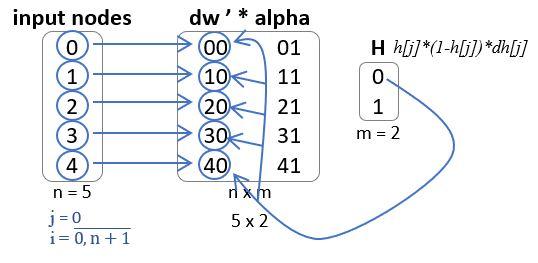
\includegraphics[width=0.48\linewidth]{azuriranje_w_.JPG}}
    \subfigure{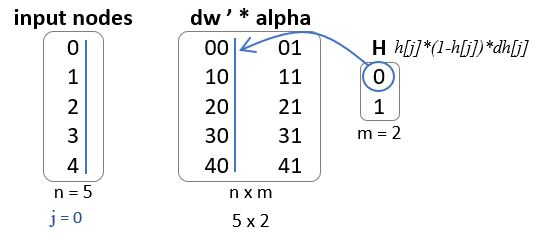
\includegraphics[width=0.48\linewidth]{poboljsano_azuriranje_w_.JPG}} 
    \caption{Ažuriranje \texttt{dw\_}. Naivni pristup sa leve strane i poboljšani sa desne.}
    \label{fig:azuriranjewp}
\end{figure}

\pagebreak
\paragraph{Azuriranje W''(jk) i deltaW''(jk)}

\begin{minted}{python}
# Naivna implementacija
for k in range(1, p):
    for j in range(0, m):
        dw__[j][k] = eta * h[j] * error + alpha * dw__[j][k]
        w__[j][k] += dw__[j][k]
\end{minted}
\texttt{dw\_\_} i \texttt{w\_} su u našem slučaju vektori pošto imamo samo jedan izlaz. Samim tim je dovoljno primeniti pokoordinatne operacije nad vektorima.
\begin{minted}{python}
# Poboljsana implementacija
dw__ *= alpha
dw__ += (eta * h * error)
w__ += dw__
\end{minted}

Ukoliko smo prošli prvu iteraciju dodajemo još jedan red u težinsku matricu \texttt{w\_} pošto nam se povećao broj ulaznih čvorova za 1.

Implementirano je čuvanje modela koji je imao najmanju \texttt{mse} tako što se upišu težinske matrice u tekstualni fajl koji je prilikom ponovnog pokretanja programa moguće učitati.

\subsection{Testiranje}
Nakon treniranja mreže ili učitavanja postojećeg modela vrši se evaluacija modela. Prolazi se kroz ceo test skup po sličnom principu po kome smo trenirali mrežu.
\begin{minted}{python}
input_nodes = concatenate(
            (bias, (x_test[day:(day+N)]).reshape(-1), output_arr))
day += 1
# Izracunavanje h1,..., hm cvorova skrivenog sloja
# U prvoj iteraciji nemamo output cvor tako da 
# ne koristimo celu w' matricu
u = []
if init_iter:
    for i in best_w_[:-1].T:
        u += [activation_f(multiply(i, input_nodes).sum())]
    init_iter = False
else:
    for i in best_w_.T:
        u += [activation_f(multiply(i, input_nodes).sum())]
h = array(u)
h[0] = 1  # bias ostaje nepromenjen

# Izracunavanje o1,...,op
o[day] = activation_f(sum(multiply(h, best_w__)))
output_arr = array([o[day]])
\end{minted}
Računa se \texttt{mean\_sqared\_error}, \texttt{mean\_absolute\_error} i prikazuje na izlazu. Generiše se grafik na kome su prikazane prave i predviđene vrednosti.

\subsection{Primeri rezultata}
Prilikom testiranja imali smo razne kombinacije, od kojih će biti prikazano par. U daljem tekstu imaćemo sledeće oznake: \texttt{n} -- broj ulaznih čvorova, \texttt{m} -- broj čvorova skrivenog sloja.
Na svakoj strani je prikazan izlaz programa za različite kombinacije parametara. Svaki grafik epohe sadrži poslednjih 365 dana u toj epohi. Isto važi i za prikaz grafika test skupa.

\\

Na graficima je crvenom bojom predstavljen skup tačnih vrednosti, a plavom su označene vrednosti predviđane programom.


\newgeometry{left=10mm, right=50mm, top=10mm, bottom=10mm, head=0mm, foot=0mm, marginpar=0mm, marginparsep=0mm, headsep=0mm}
\pagebreak % -------------------------------------------------------------- MODEL
\subsubsection{Model \texttt{n = 54, m = 270, alpha = 0.5, eta = 0.3}}
\begin{figure}[h!]
\begin{center}
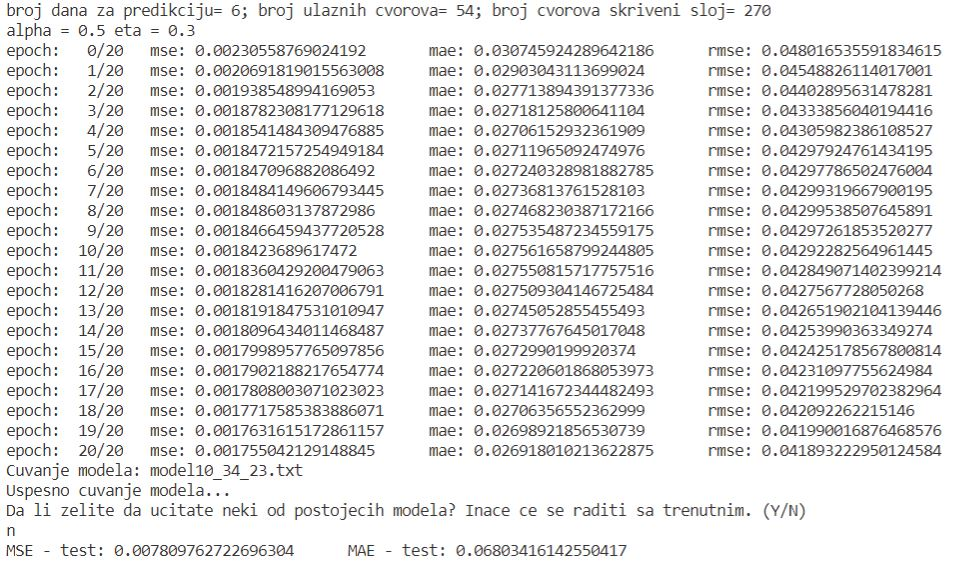
\includegraphics[scale=0.9]{output/output_example_program_10_34_23.JPG}
\end{center}
\caption{Output programa za parametre \texttt{m = 270, alpha = 0.5, eta = 0.3}}
\end{figure}
\begin{figure}[h!]
    \centering
    \subfigure{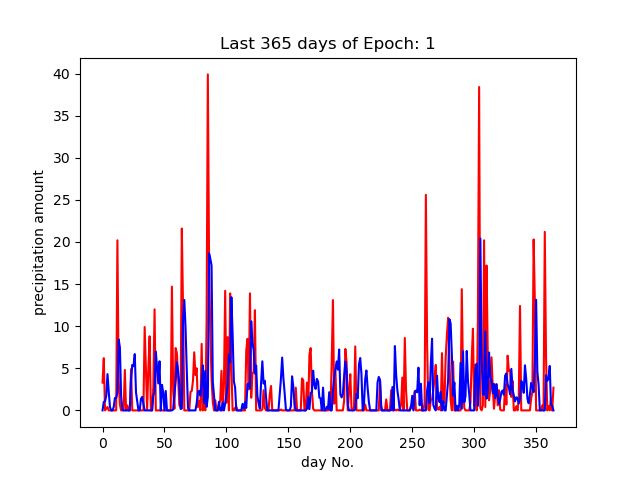
\includegraphics[width=0.49\linewidth]{plots/plot_epoch_1_time_10_34_23.png}} 
    \subfigure{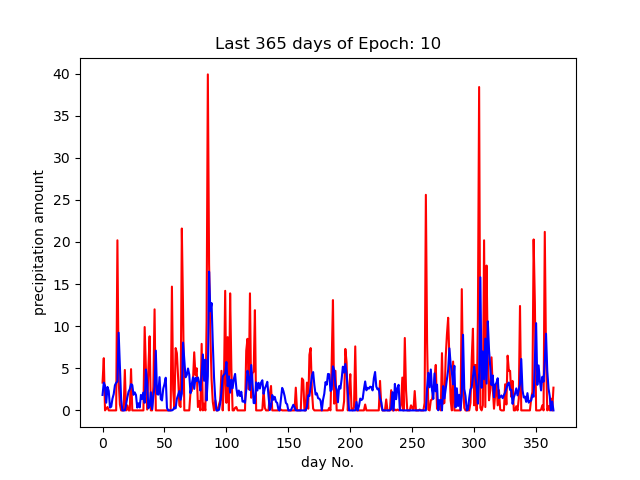
\includegraphics[width=0.49\linewidth]{plots/plot_epoch_10_time_10_34_23.png}} 
    \subfigure{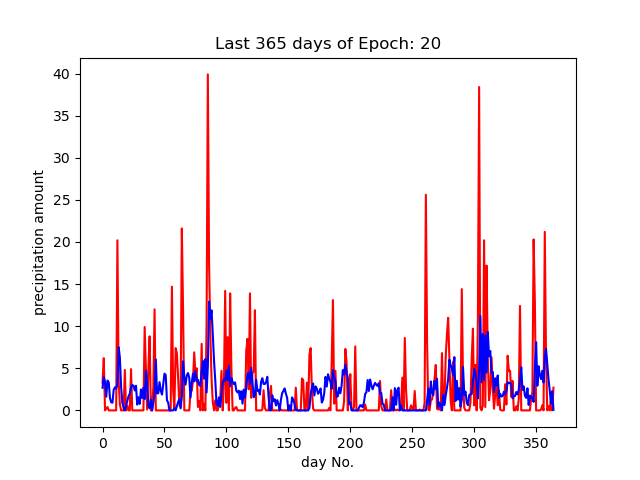
\includegraphics[width=0.49\linewidth]{plots/plot_epoch_20_time_10_34_23.png}}
    \subfigure{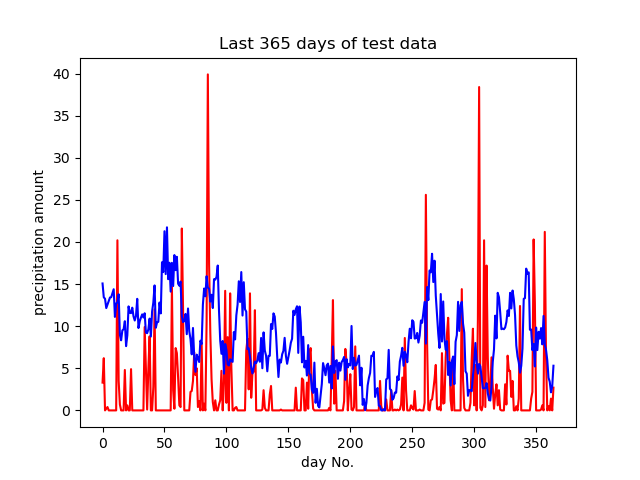
\includegraphics[width=0.49\linewidth]{plots/plot_test_model-model10_34_23-time_10_34_23.png}}
    \caption{Grafici za parametre \texttt{m = 270, alpha = 0.5, eta = 0.3}}
\end{figure}

\pagebreak % -------------------------------------------------------------- MODEL
\subsubsection{Model \texttt{n = 54, m = 270, alpha = 0.2, eta = 0.3}}
\begin{figure}[h!]
\begin{center}
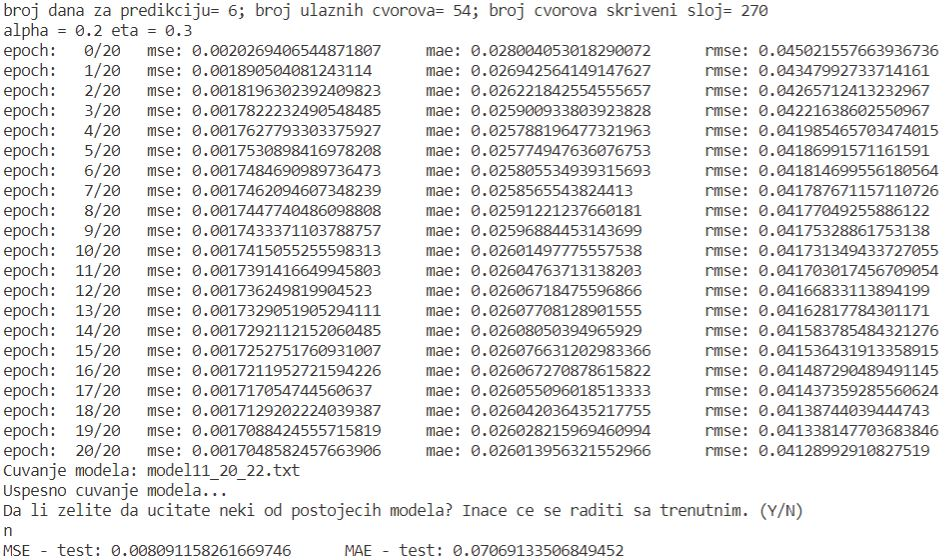
\includegraphics[scale=0.9]{output/output_example_program_11_20_22.JPG}
\end{center}
\caption{Output programa za parametre \texttt{m = 270, alpha = 0.2, eta = 0.3}}
\end{figure}
\begin{figure}[h!]
    \centering
    \subfigure{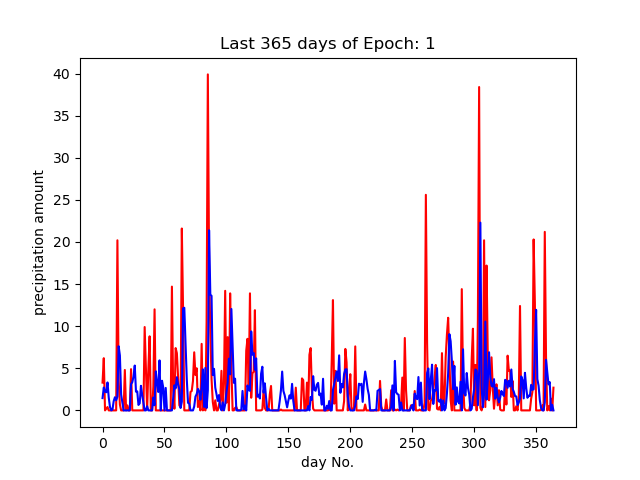
\includegraphics[width=0.49\textwidth]{plots/plot_epoch_1_time_11_20_22.png}} 
    \subfigure{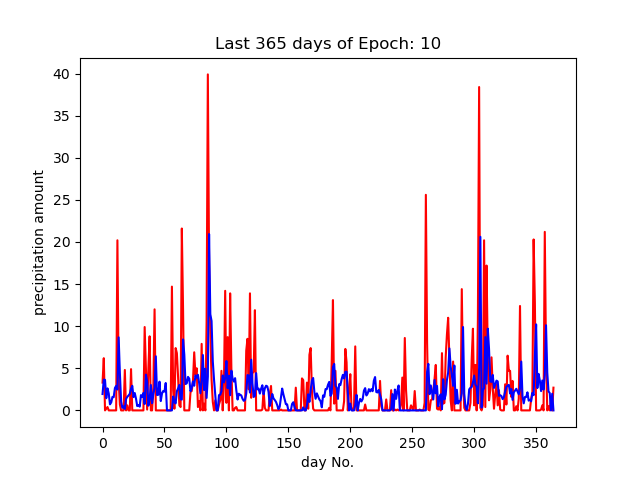
\includegraphics[width=0.49\textwidth]{plots/plot_epoch_10_time_11_20_22.png}} 
    \subfigure{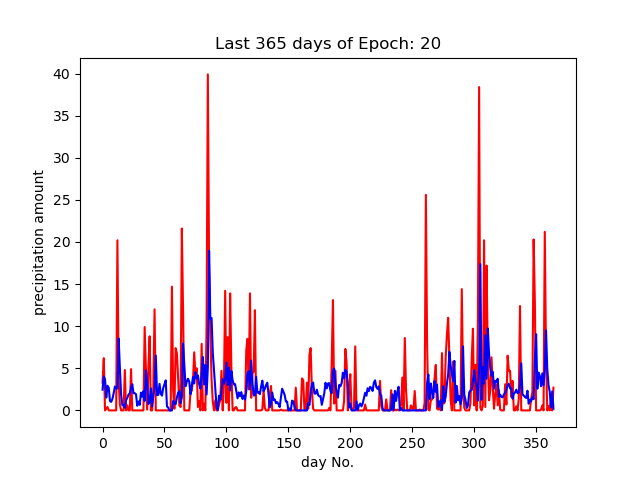
\includegraphics[width=0.49\textwidth]{plots/plot_epoch_20_time_11_20_22.png}}
    \subfigure{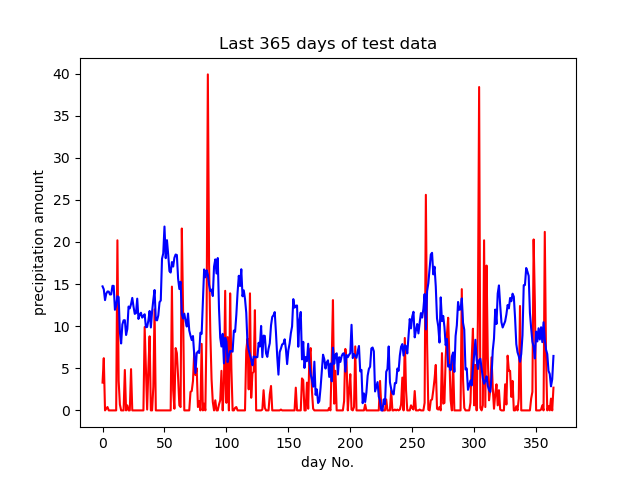
\includegraphics[width=0.49\textwidth]{plots/plot_test_model-model11_20_22-time_11_20_22.png}}
    \caption{Grafici za parametre \texttt{m = 270, alpha = 0.2, eta = 0.3}}
\end{figure}

\pagebreak % -------------------------------------------------------------- MODEL
\subsubsection{Model \texttt{n = 54, m = 108, alpha = 0.2, eta = 0.3}}
\begin{figure}[h!]
\begin{center}
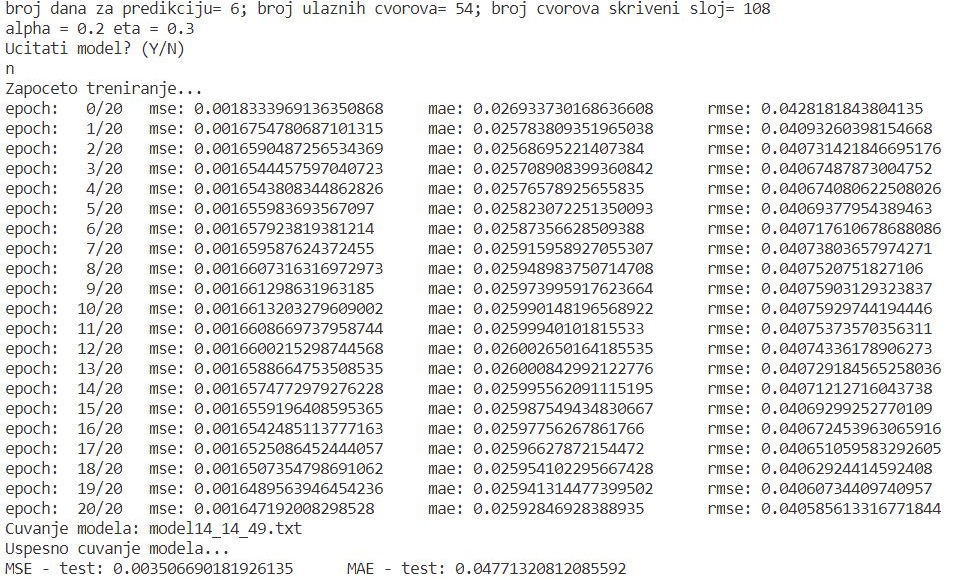
\includegraphics[scale=0.9]{output/output_example_program_14_14_49.JPG}
\end{center}
\caption{Output programa za parametre \texttt{n = 54, m = 108, alpha = 0.2, eta = 0.3}}
\end{figure}

\begin{figure}[h!]
    \centering
    \subfigure{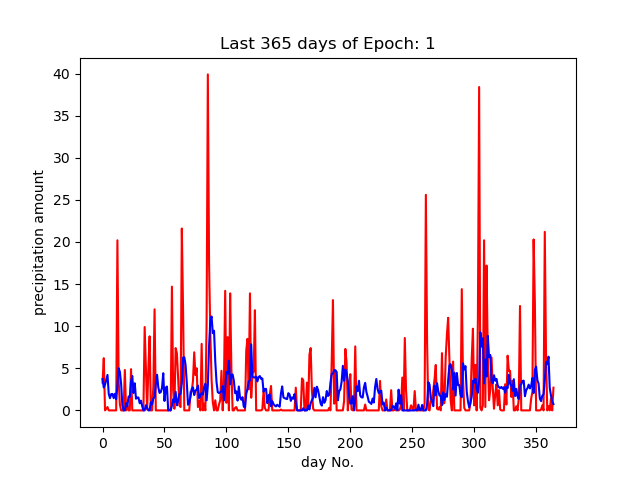
\includegraphics[width=0.49\textwidth]{plots/plot_epoch_1_time_14_14_49.png}} 
    \subfigure{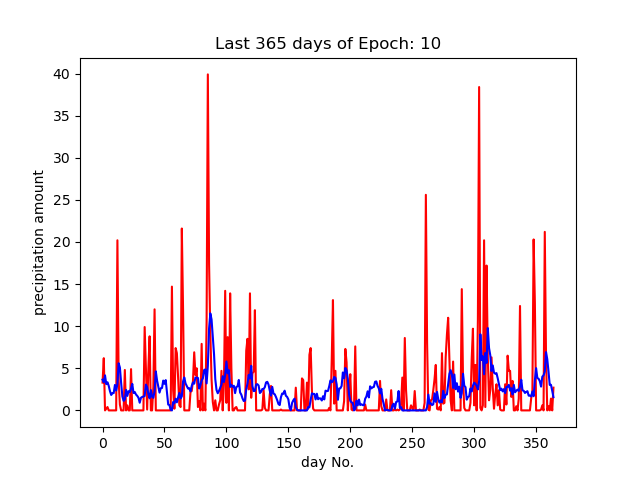
\includegraphics[width=0.49\textwidth]{plots/plot_epoch_10_time_14_14_49.png}} 
    \subfigure{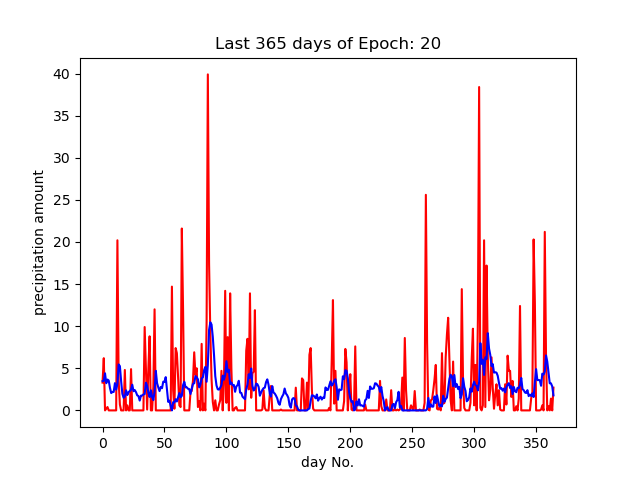
\includegraphics[width=0.49\textwidth]{plots/plot_epoch_20_time_14_14_49.png}}
    \subfigure{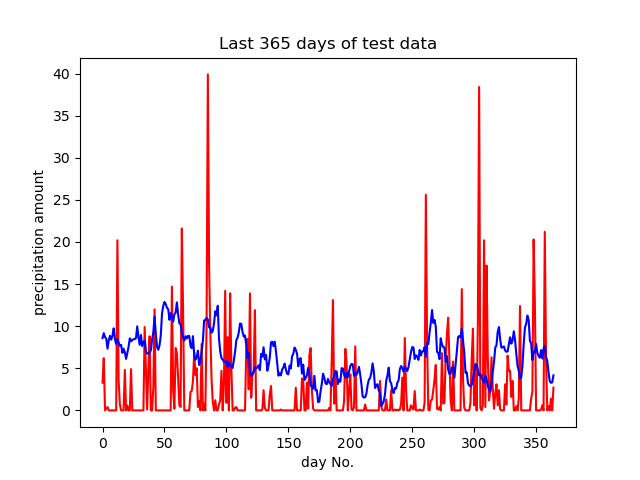
\includegraphics[width=0.49\textwidth]{plots/plot_test_model-model14_14_49-time_14_14_49.png}}
    \caption{Grafici za parametre \texttt{n = 54, m = 108, alpha = 0.2, eta = 0.3}}
\end{figure}

\pagebreak % -------------------------------------------------------------- MODEL
\subsubsection{Model \texttt{n = 54, m = 108, alpha = 0.9, eta = 0.5}}
\begin{figure}[h!]
\begin{center}
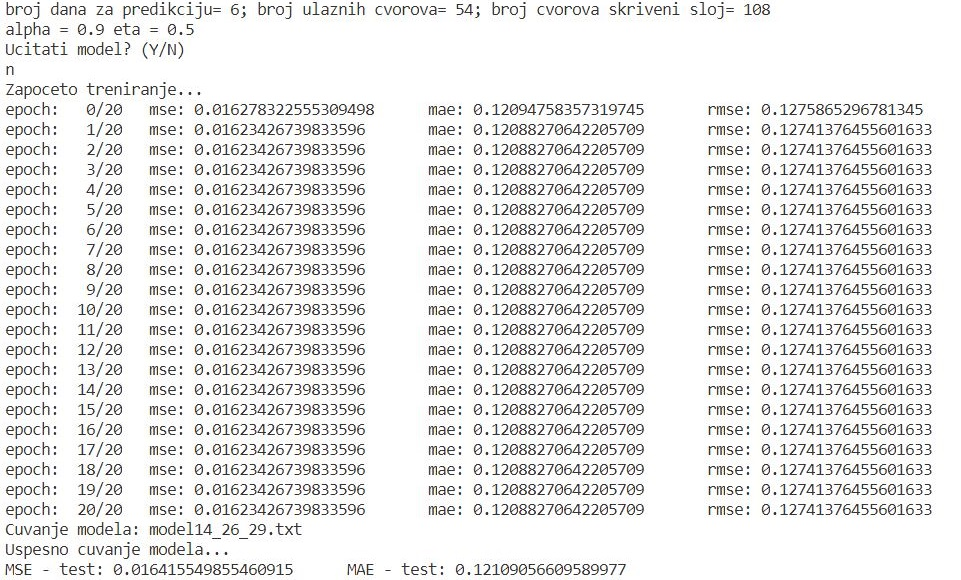
\includegraphics[scale=0.9]{output/output_example_program_14_26_29.JPG}
\end{center}
\caption{Output programa za parametre \texttt{m = 108, alpha = 0.9, eta = 0.5}}
\end{figure}
\begin{figure}[h!]
    \centering
    \subfigure{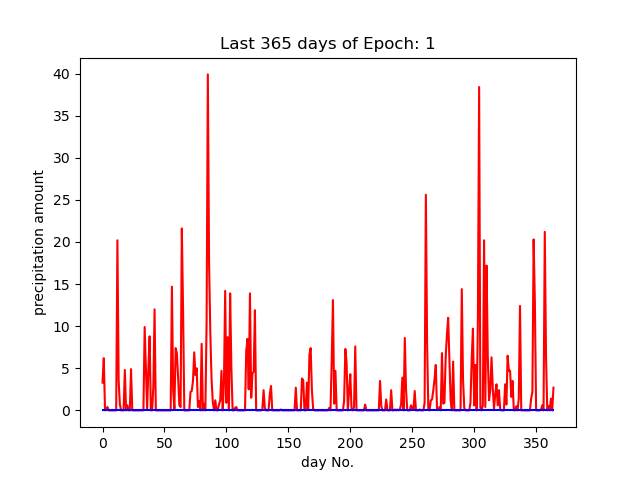
\includegraphics[width=0.49\textwidth]{plots/plot_epoch_1_time_14_26_29.png}} 
    \subfigure{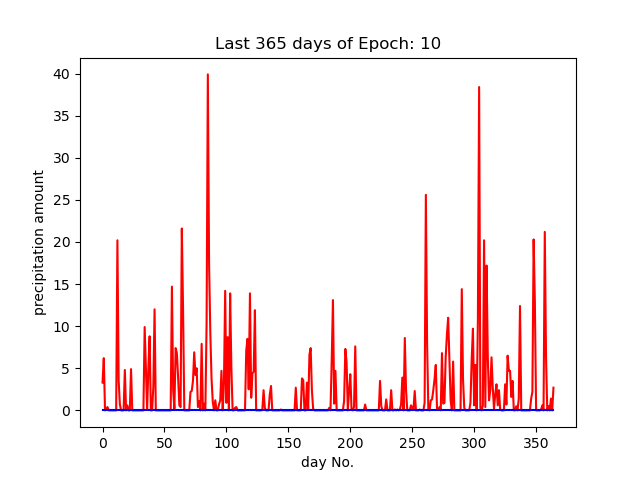
\includegraphics[width=0.49\textwidth]{plots/plot_epoch_10_time_14_26_29.png}} 
    \subfigure{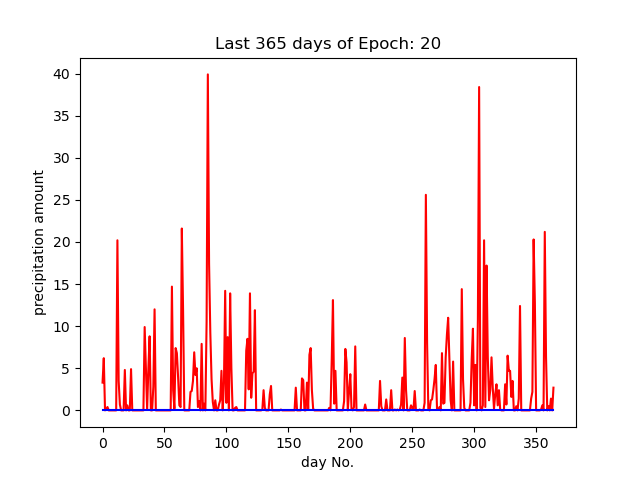
\includegraphics[width=0.49\textwidth]{plots/plot_epoch_20_time_14_26_29.png}}
    \subfigure{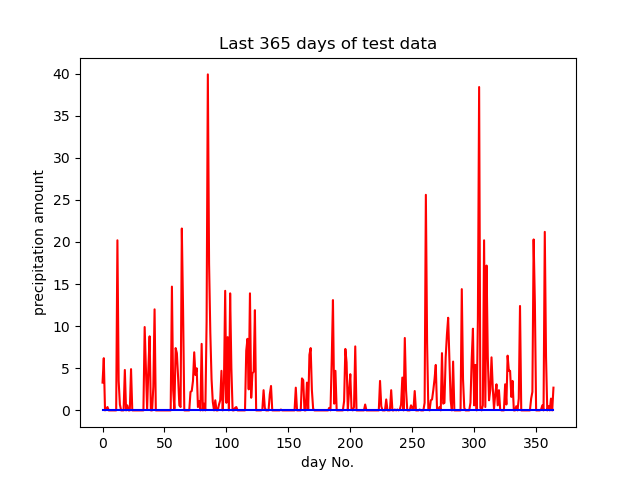
\includegraphics[width=0.49\textwidth]{plots/plot_test_model-model14_26_29-time_14_26_29.png}}
    \caption{Grafici za parametre \texttt{m = 108, alpha = 0.9, eta = 0.5}}
\end{figure}

\pagebreak % -------------------------------------------------------------- MODEL
\subsubsection{Model \texttt{n = 54, m = 216, alpha = 0.2, eta = 0.3}}
\begin{figure}[h!]
\begin{center}
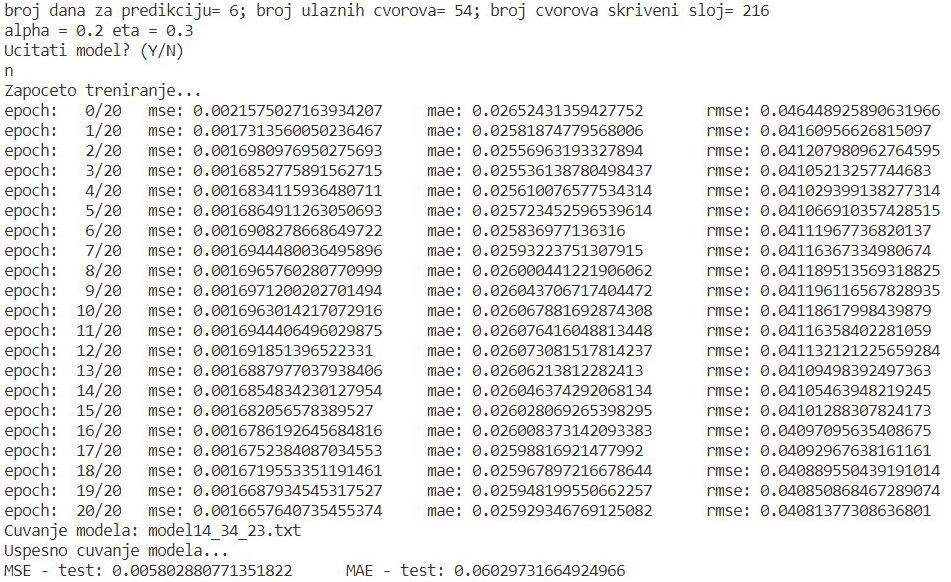
\includegraphics[scale=0.9]{output/output_example_program_14_34_23.JPG}
\end{center}
\caption{Output programa za parametre \texttt{m = 216, alpha = 0.2, eta = 0.3}}
\end{figure}

\begin{figure}[h!]
    \centering
    \subfigure{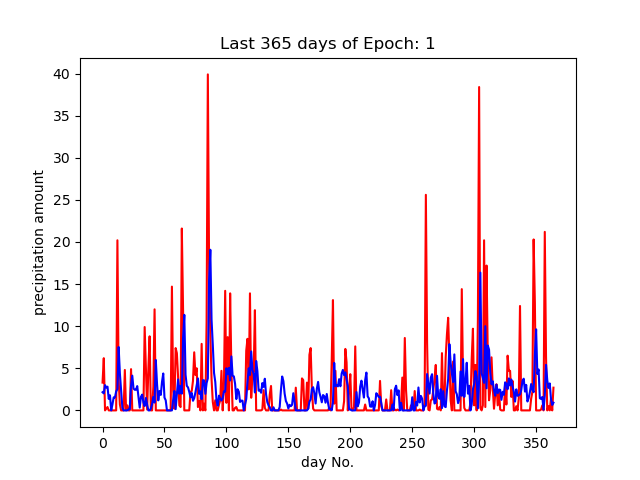
\includegraphics[width=0.49\textwidth]{plots/plot_epoch_1_time_14_34_23.png}} 
    \subfigure{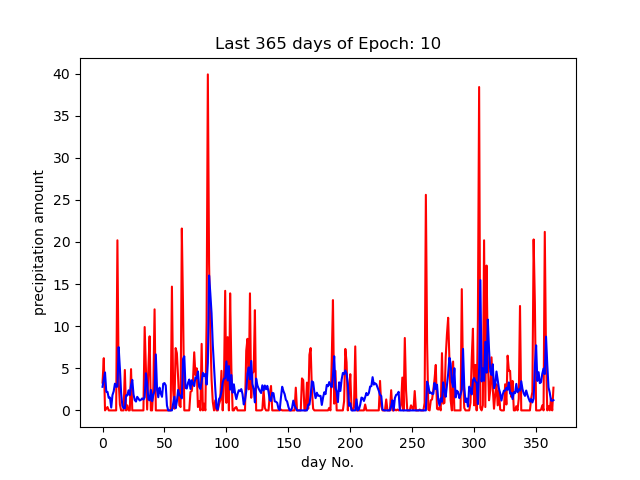
\includegraphics[width=0.49\textwidth]{plots/plot_epoch_10_time_14_34_23.png}} 
    \subfigure{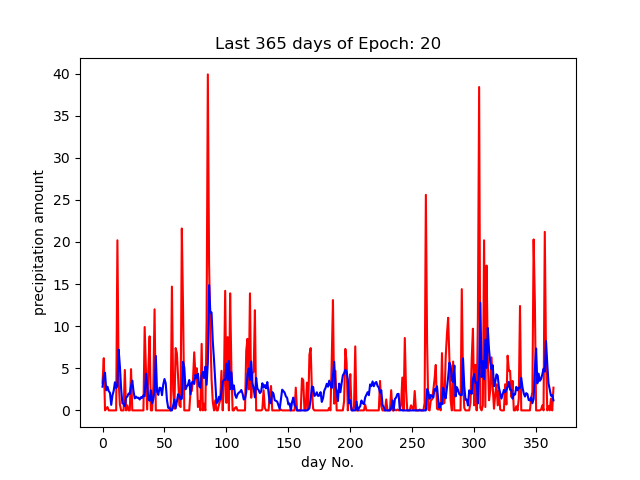
\includegraphics[width=0.49\textwidth]{plots/plot_epoch_20_time_14_34_23.png}}
    \subfigure{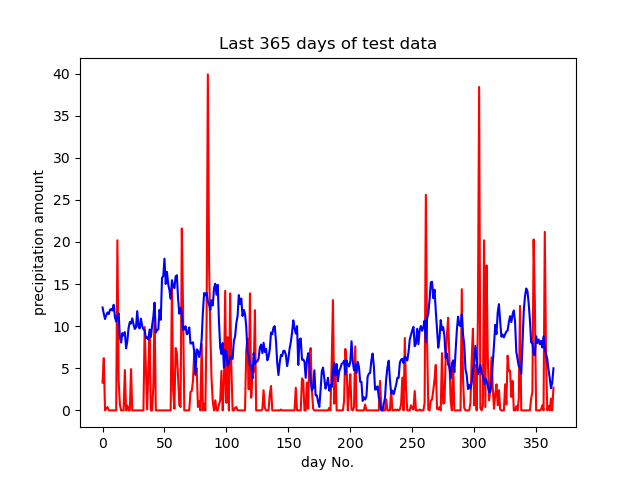
\includegraphics[width=0.49\textwidth]{plots/plot_test_model-model14_34_23-time_14_34_23.png}}
    \caption{Grafici za parametre \texttt{m = 216, alpha = 0.2, eta = 0.3}}
\end{figure}

\pagebreak

\restoregeometry
\section{Zaključak}

Prema prikazanim modelima primećujemo da iako su greške modela sa različitim parametrima približne, maltene iste, nakon skaliranja podataka u njihov originalni rang vrednosti vidi se koliko je zapravo loše predviđano. 
Za veći broj čvorova u skrivenom sloju model uspeva da se donekle približi ekstremima, dok se za manji broj to ne postiže. Za velike vrednosti $\alpha$ prebrzo ode u minimum i ne može da se povrati iz njega. U odnosu na test skup svi modeli su se podjenako loše pokazali. Na nepoznatim podacima nije efikasan, ali za uzastopne podatke se može reći da donekle uspeva da predvidi naredne vrednosti.

Model treniran ovakvim algoritmom koji uzima u obzir samo jedan skriveni sloj je efikasniji za jednostavnije probleme predviđanja, tako da bi naredni korak u poboljšanju algoritma bio dodavanje jos jednog skrivenog sloja i više eksperimentisanja sa parametrima.

\addcontentsline{toc}{section}{Literatura}
\appendix
\bibliography{seminarski} 
\bibliographystyle{plain}

% \appendix
% \section{Dodatak}


\end{document}
